% !TeX spellcheck = en_US
%% 
%% Copyright 2007-2020 Elsevier Ltd
%% 
%% This file is part of the 'Elsarticle Bundle'.
%% ---------------------------------------------
%% 
%% It may be distributed under the conditions of the LaTeX Project Public
%% License, either version 1.2 of this license or (at your option) any
%% later version.  The latest version of this license is in
%%    http://www.latex-project.org/lppl.txt
%% and version 1.2 or later is part of all distributions of LaTeX
%% version 1999/12/01 or later.
%% 
%% The list of all files belonging to the 'Elsarticle Bundle' is
%% given in the file `manifest.txt'.
%% 
%% Template article for Elsevier's document class `elsarticle'
%% with harvard style bibliographic references

%\documentclass[preprint,12pt,authoryear]{elsarticle}

%% Use the option review to obtain double line spacing
%% \documentclass[authoryear,preprint,review,12pt]{elsarticle}

%% Use the options 1p,twocolumn; 3p; 3p,twocolumn; 5p; or 5p,twocolumn
%% for a journal layout:
%% \documentclass[final,1p,times,authoryear]{elsarticle}
%% \documentclass[final,1p,times,twocolumn,authoryear]{elsarticle}
%% \documentclass[final,3p,times,authoryear]{elsarticle}
%% \documentclass[final,3p,times,twocolumn,authoryear]{elsarticle}
%% \documentclass[final,5p,times,authoryear]{elsarticle}
 \documentclass[final,5p,times,twocolumn,authoryear]{elsarticle}

%% For including figures, graphicx.sty has been loaded in
%% elsarticle.cls. If you prefer to use the old commands
%% please give \usepackage{epsfig}

%% The amssymb package provides various useful mathematical symbols
\usepackage{amsmath,amsfonts,amssymb,amscd,amsthm,xspace,bm}
\usepackage{mathtools}
\usepackage{lipsum}
\usepackage[pdfpagemode={UseOutlines},bookmarks=true,bookmarksopen=true,
bookmarksopenlevel=0,bookmarksnumbered=true,hypertexnames=false,
colorlinks,linkcolor={blue},citecolor={blue},urlcolor={red},
pdfstartview={FitV},unicode,breaklinks=true]{hyperref}
\usepackage{derivative}
\usepackage{siunitx}
\sisetup{
	display-per-mode=fraction,
	inline-per-mode=power,
	separate-uncertainty,
	separate-uncertainty-units=single,
	list-final-separator=و,
	list-pair-separator=و,
	range-phrase=تا
}
\usepackage{datatool}
\usepackage{cancel}
\usepackage{graphicx,subfigure,wrapfig}
\usepackage{color}
\usepackage{pifont}
%% The amsthm package provides extended theorem environments
%% \usepackage{amsthm}

%% The lineno packages adds line numbers. Start line numbering with
%% \begin{linenumbers}, end it with \end{linenumbers}. Or switch it on
%% for the whole article with \linenumbers.
%% \usepackage{lineno}

%% You might want to define your own abbreviated commands for common used terms, e.g.:

\journal{Dr. Amin Faraji}


\begin{document}

\begin{frontmatter}

%% Title, authors and addresses

%% use the tnoteref command within \title for footnotes;
%% use the tnotetext command for theassociated footnote;
%% use the fnref command within \author or \affiliation for footnotes;
%% use the fntext command for theassociated footnote;
%% use the corref command within \author for corresponding author footnotes;
%% use the cortext command for theassociated footnote;
%% use the ead command for the email address,
%% and the form \ead[url] for the home page:
%% \title{Title\tnoteref{label1}}
%% \tnotetext[label1]{}
%% \author{Name\corref{cor1}\fnref{label2}}
%% \ead{email address}
%% \ead[url]{home page}
%% \fntext[label2]{}
%% \cortext[cor1]{}
%% \affiliation{organization={},
%%            addressline={}, 
%%            city={},
%%            postcode={}, 
%%            state={},
%%            country={}}
%% \fntext[label3]{}

\title{Exploring Periodic Boundary Conditions: A Study on 2D and 3D Spheres and Continuum Limit}

%% use optional labels to link authors explicitly to addresses:
%% \author[label1,label2]{}
%% \affiliation[label1]{organization={},
%%             addressline={},
%%             city={},
%%             postcode={},
%%             state={},
%%             country={}}
%%
%% \affiliation[label2]{organization={},
%%             addressline={},
%%             city={},
%%             postcode={},
%%             state={},
%%             country={}}

\author[first]{Alireza Same}
\fntext[first]{99100709}
\ead{alirezasame@gmail.com}
\author[second]{Hanie Hatami}
\fntext[second]{99100614}
\ead{alirezasame@gmail.com}
\author[third]{Mehrnaz Rabiee}
\fntext[third]{99100669}
\ead{alirezasame@gmail.com}

\begin{abstract}
%% Text of abstract
We analyze systems with periodic boundary conditions in two and three dimensions. Beginning with an $N$-particle system confined to a circle, we derive the governing ordinary differential equation and solve it both analytically using circulant matrices and numerically. We then take the continuum limit as $N$ goes to infinity to obtain a wave equation on the circle with periodic boundary conditions. This partial differential equation is solved exactly, allowing us to construct visualizations of the propagating waves. Next we study an $N$-particle system confined to the surface of a regular polyhedron, deriving the discrete equations and solving numerically using symmetry arguments. We then discuss statistical mechanics approaches for this system. Finally, we analyze longitudinal elastic waves propagating on a sphere, deriving the continuum wave equation in spherical coordinates and discussing analytical and numerical solution methods based on spectral decomposition. Throughout we emphasize the mathematical physics, solving equations analytically where possible and numerically otherwise. Results for all systems are illustrated through figures.
\end{abstract}

%%Graphical abstract
%\begin{graphicalabstract}
%\includegraphics{grabs}
%\end{graphicalabstract}

%%Research highlights
%\begin{highlights}
%\item Research highlight 1
%\item Research highlight 2
%\end{highlights}

\begin{keyword}
%% keywords here, in the form: keyword \sep keyword, up to a maximum of 6 keywords
Particle Systems \sep Mathematical Physics \sep Fourier Analysis \sep Differential Equations \sep Continuum Limit \sep Periodic Symmetry \sep Platonic Solids

%% PACS codes here, in the form: \PACS code \sep code

%% MSC codes here, in the form: \MSC code \sep code
%% or \MSC[2008] code \sep code (2000 is the default)

\end{keyword}


\end{frontmatter}

%\tableofcontents

%% \linenumbers

%% main text

\section{Introduction}
\label{introduction}
Periodic boundary conditions arise naturally in the study of waves and particles constrained to closed topologies. The mathematics of such systems, though conceptually simple, reveals rich physical behaviors. In one dimension, systems with periodic boundaries can be solved exactly. As the dimension increases, new challenges emerge. On a circle, the topology is uniform and easily parametrized, yielding to straightforward analysis via Fourier decomposition. On a sphere, the additional dimension introduces variability in the surface curvature, requiring more advanced methods like spherical harmonics. In three dimensions, modeling particles or waves constrained to regular convex polyhedron brings deeper obstacles, as these Platonic solids resist exact geometric parameterization.

Approximation methods must therefore complement exact mathematical techniques in exploring these systems. The interplay of analytical, numerical, and geometric ideas is what makes periodic systems fascinating to study. When symmetry allows clean solutions, the mathematics elegantly explains the physics. And when intricacies of higher dimensions obstruct analysis, numerical methods and geometric intuition guide the way.

In this Article, we embark on a mathematical tour of periodic boundaries in multiple dimensions. We begin with approachable problems, deriving and solving ordinary differential equations through matrix techniques. Moving to continuous systems, we encounter tractable partial differential equations which yield to Fourier analysis. Finally, we contend with intricate geometries, wrestling with equations which only numerical computation can conquer. What ties these investigations together is the quest to understand systems constrained to live within themselves, endowed with a symmetry as beautiful as it is challenging.

\section{2D Spheres Revisited}
\label{sec-2D}
\subsection{Analytical Description}
As established in foundational texts on wave phenomena (see \cite{georgiPhysicsWaves2015}), a prototypical model for cyclic wave propagation considers a discrete set of point particles confined to a circular domain. This framework relies on two key approximations: first, that interactions are strictly local, with each particle only directly influencing its immediate neighbors. Second, that the inter-particle forces respond linearly to changes in separation relative to an equilibrium length. While undeniably reductionist, these assumptions prove sufficient to capture the salient physics of transverse wave transmission through the medium.

Specifically, we examine a system of $N$ identical particles of mass $m$ regularly spaced around a ring of radius $R$. Identical harmonic springs, characterized by force constant $k$, link adjacent particles along the circumference. This geometry exhibits a continuous rotational symmetry - rotations and reflections by $2\pi/N$ map the configuration onto itself. Our theoretical description should therefore not differentiate between the $2N$ symmetry-equivalent orientations. The sole measurable degree of freedom lies in the particles' relative displacements, as absolute positions along the circle can not be experimentally determined without first arbitrarily fixing a reference point.

The simplicity of this model, alongside its inherent periodicity, motivate its study before tackling more intricate geometries in higher dimensions. Even within the confines of localized, linear interactions, analytical and computational techniques reveal rich wave behaviors arising from the cyclic topology. The mathematics provides profound and elegant insight into the underlying physics.

As an elementary example, Figure \ref{fig-n4} illustrates the case for $N=4$ particles. The fourfold rotational symmetry is evident, as is the periodic nature of the circular boundary. With the model established, we now embark on an in-depth analysis.

\begin{figure}[h]
	\centering 
	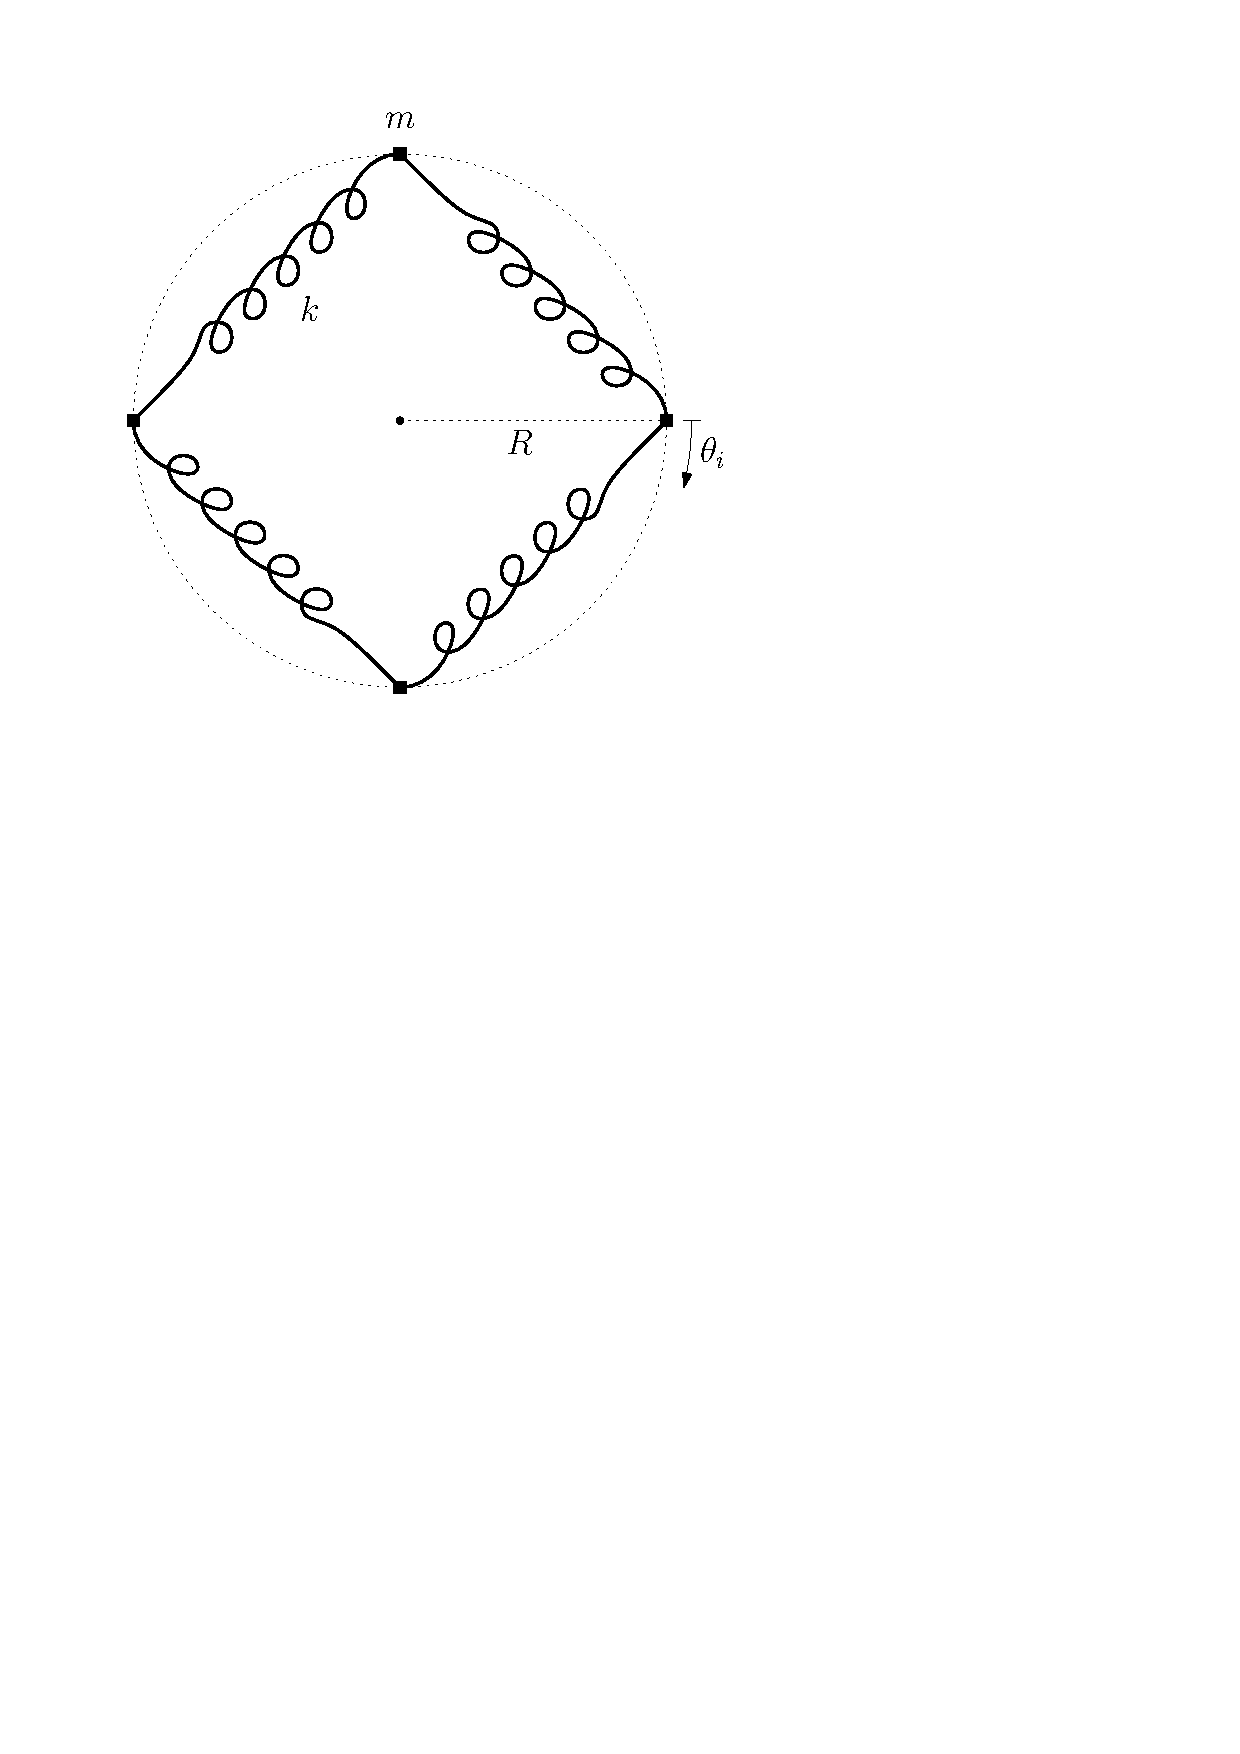
\includegraphics[width=0.25\textwidth]{../Figures/1D-4Particle-Springs.pdf}	
	\caption{4 identically distributed point masses on a circle} 
	\label{fig-n4}
\end{figure}

The configuration of the system can be fully specified by the central angle displacement $\theta_i$ of each particle $i$ relative to its initial angular position. As per the rotational symmetry, the labeling of individual particles carries no physical significance. We therefore characterize the state through the $N$-dimensional vector $\bm{\theta} = (\theta_1, \theta_2, ..., \theta_N)$ encompassing each particle's angular shift. For small oscillations, we expect the time evolution of $\bm{\theta}$ to follow a linear equation of the form:

\begin{equation}
	M\ddot{\bm{\theta}} + K\bm{\theta} = 0 \Rightarrow \ddot{\bm{\theta}} + W\bm{\theta} = 0
	\label{eq-funda}
\end{equation}

The matrix $W$ belongs to the special class of circulant matrices which respect circular permutation symmetry. To derive its structure, consider the $i$th particle's interactions: since it only couples to its nearest neighbors, its motion is governed by:

\begin{equation*}
	\ddot{\theta}_i = a \theta_{i-1} + b \theta_i + c \theta_{i+1}
\end{equation*}

By symmetry, the coefficient $a$ equals $c$. For a system of $N$ particles, this yields an interaction matrix $W$ of the form:

\begin{equation}
	W =
	\begin{pmatrix}
		A & B & 0 & \dots & B \\
		B & A & B & \dots & 0 \\
		
		0 & B & A & \dots & 0 \\
		\vdots & \vdots & \vdots & \ddots & \vdots \\
		B & 0 & 0 & \dots & A
	\end{pmatrix}_{N \times N}
	\label{eq-Wcirculant}	
\end{equation}

While the precise values of $A$ and $B$ do not qualitatively impact the dynamics, specific models may impose further constraints such as $A = -2B$ (see \cite{georgiPhysicsWaves2015}). Analytical solutions rely on the circulant structure, as discussed in \cite{grayToeplitzCirculantMatrices2006}.

As discussed, the normal modes of this system should respect the circular symmetry. This mandates mode shapes of the form:
\begin{equation*}
	\bm{\beta}^{(k)} = \left(1, \omega^k, \omega^{2k},\dots, \omega^{N-1}\right) \qquad \omega = e^{2\pi i/N}
\end{equation*}  
where $\omega$ denotes the complex $N$th root of unity. The angular frequency $\omega_k$ of the $k$th mode takes the form:
\[ \omega_k^2=A + 2B\cos\left(\frac{2k\pi}{N}\right) \qquad k = 0,1,\dots, N-1 \]
This reveals intrinsic degeneracies arising from the system's symmetry. For even $N$, the $k=0$ and $k=N/2$ modes have real-valued eigenvectors, while the remaining $N-2$ modes come in complex-conjugate pairs which can be combined into degenerate real modes. The connection to Fourier analysis will become transparent in examining the continuum limit. The normal modes indeed correspond to a Discrete Fourier Transform, as elaborated in \cite{grayToeplitzCirculantMatrices2006}. The circulant structure enables analytical decomposition into these symmetry-dictated eigenmodes.

In the Case where $A=-2B $ the relation simplifies to the simpler case below:
\[ \omega_k^2 = \omega_0^2\sin^2\left(\frac{k\pi}{N}\right) \]

\subsection{Numerical Description and Comparison with the Analytical Solution}
Thus far, we have relied on linearized equations to enable an analytical treatment. To complement this, we now numerically simulate the full nonlinear particle interactions without simplifications. Details of the model and algorithms are in the supplementary simulation \href{https://github.com/a-samea/Waves-CourseProject/blob/main/Simulations/N%20Particle.ipynb}{Jupyter Notebook}. In short, we integrate the coupled second-order ODEs for the $N$ particles using an adaptive timestep fourth-order Runge-Kutta Python routine. By systematically increasing the imposed oscillation amplitude, we can validate the accuracy of our small amplitude analytical solutions and probe changes at higher displacements. These computations provide a flexible framework to incorporate future refinements like stochastic forces or dissipation. Most importantly, the nonlinear simulations both test the assumptions made earlier and better represent the true dynamics.

\subsection{Continuum Limit}
In taking the continuum limit, the number of particles $N$ approaches infinity, transforming the discrete mechanical system into a continuous cyclic domain. Our coordinate $\varphi$ becomes a continuous angular variable, with the wave displacement $u(\varphi,t)$ encapsulating the discrete particle shifts $\theta_j(t) $ through:
\[ u(\varphi_j,t) = \theta_j(t) \quad \text{where:} \quad \varphi_j=\frac{2\pi j}{N} \quad j = 0,\dots,N-1 \]
As $N$ tends to infinity, $\varphi_j$ transitions to a smooth continuous coordinate $\varphi$. The partial differential wave equation governing disturbances naturally emerges from the initial discrete equations of motion (Equation \ref{eq-funda}):
\begin{equation}
	\pdv[order={2}]{u}{t} = c^2 \pdv[order={2}]{u}{\varphi}, \quad u(\varphi,t) = u(\varphi+2\pi,t)
	\label{eq-waveperiodic}
\end{equation}

The wave velocity $c$ descending directly from the interaction matrix elements $W$ reflects intrinsic timescales rather than typical speeds. More profoundly, the periodic continuity condition connecting values of $u $ at $\varphi$ and $\varphi+2\pi$ represents the imprint of the cyclic group symmetry. This maintenance of key features accompanies the facilitation of an analytical treatment of waves on the smooth circle.

We can solve this equation (\ref{eq-waveperiodic}) by separation of variables. if we assume the form below for the disturbance the wave equation becomes:
\[ u(\varphi,t) = \phi(\varphi)\tau(t) \Rightarrow \frac{1}{c^2\tau}\odv[order={2}]{\tau}{t} = \frac{1}{\phi}\odv[order={2}]{\phi}{\varphi}, \quad \phi(\varphi) = \phi(\varphi+2\pi) \]
The SLODEs above have the periodic boundary condition imposed on the part involving $\varphi$. So each part can only be a negative constant which respects periodic conditions:
\begin{align}
	\odv[order={2}]{\phi}{\varphi} + m^2 \phi =0 &\Rightarrow m = 0 , 1 , 2 , \dots \label{eq-restrictions} \\
	\odv[order={2}]{\tau}{t} + m^2c^2 \tau =0 &\Rightarrow \tau(t) = C_1 \cos\left(mct\right) + C_2 \sin(mct) \label{eq-timepart}
\end{align}
Also, the time translation invariance implies that there is no preferred phase for the time factor that cannot be considered in the angle factor. So, we can represent Eigenstates of the PDE by the following functions:
\begin{align*}
	& u_0(\varphi,t) = u_0 \\
	& u_m(\varphi,t) = \left[a_m \cos(m\varphi) + b_m\cos(m\varphi)\right]\cos(mct+\theta_m)
\end{align*}
The set above creates a complete orthogonal set of answers for the wave equation \ref{eq-waveperiodic} respecting the periodic boundary conditions. As it turns out, the equation below is completely solved (see \cite{evansPartialDifferentialEquations2022}) and has some beatiful remarks.
\begin{equation}
	\label{eq-fullwave}\begin{aligned}
		& \pdv[order={2}]{u}{t} = c^2 \pdv[order={2}]{u}{\varphi} \\
		& u(\varphi,t) = u(\varphi+2\pi,t) \\
		& u(\varphi,0) = f(\varphi) = f(\varphi + 2\pi) \\
		& \dot{u}(\varphi,0) = g(\varphi + 2\pi)
	\end{aligned}
\end{equation}
What is fascinating about the continuum limit is that the completely alternating case does not happen anymore and it is not an eigenmode. As you may recall we had the first normal mode in the discrete case with zero frequency. this is exactly $u_0$. The equation \ref{eq-fullwave} is fully solvable in a closed form. But for sake of simplicity we require $g(\varphi) = 0$ (i.e. initial velocity is zero). Then all $\theta_m$ will become zero and the coefficients are simply the Fourier Series of function $f$. i.e.:
\begin{equation}
	\begin{aligned}
		&u_0 = \frac{1}{2\pi}\int_{0}^{2\pi}f(\varphi)\odif{\varphi} \\
		&a_m = \frac{1}{\pi}\int_{0}^{2\pi}f(\varphi)\cos(m\varphi)\odif{\varphi} \\
		&b_m = \frac{1}{\pi}\int_{0}^{2\pi}f(\varphi)\sin(m\varphi)\odif{\varphi}
	\end{aligned}
\end{equation}

We can now appreciate the power of Fourier Series in this part. it is astonishing that even the couple degenerate Eigenvalues that we encountered previously are present here and for every non-zero $m$ we have two Eigenmodes. This is another reason why the alternating case does not exist in continuum limit. just because infinity is neither even nor odd and the alternating mode only happened in the even case. Another notable fact is that we had a relation between the number of mode and its angular velocity. Here we will replace some terms in it to make it compliant with continuous case. we would call such relation the \textit{Dispersion Relation} of system.
\[ \omega_k^2 = \omega_0^2\sin^2\left(\frac{k\pi}{N}\right), \quad N \gg 1 \Rightarrow \omega_k \approx \omega_0 \frac{k\pi}{N} = mc \]
Evidently the angular frequency of the mode $m$ is now given by the much simpler relation below:
\begin{equation}
	\omega_m = m c ,\qquad m = 0,1,2,\dots
\end{equation}


\section{Discussion}
%%\label{}

\section{Summary and conclusions}
%%\label{}


\section*{Acknowledgements}
Thanks to ...

%% The Appendices part is started with the command \appendix;
%% appendix sections are then done as normal sections

%% If you have bibdatabase file and want bibtex to generate the
%% bibitems, please use
%%
\bibliographystyle{elsarticle-harv} 
\bibliography{zotero}

%% else use the following coding to input the bibitems directly in the
%% TeX file.

%%\begin{thebibliography}{00}

%% \bibitem[Author(year)]{label}
%% For example:

%% \bibitem[Aladro et al.(2015)]{Aladro15} Aladro, R., Martín, S., Riquelme, D., et al. 2015, \aas, 579, A101


%%\end{thebibliography}

\end{document}

\endinput
%%
%% End of file `elsarticle-template-harv.tex'.
